
\section{Correlation of Passes and Program Features} 

\label{sec:features}
%Among the major challenges that occur when applying machine learning techniques to solve different challenging problems is the
Similar to the case with many deep learning approaches, explainability is one of the major challenges we face when applying deep RL to the phase-ordering challenge. To analyze and understand the correlation of passes and program features, we use random forests~\cite{breiman2001random} to learn the importance of different features. Random forest is an ensemble of multiple decision trees. 
%that are used to make decisions on data. 
The prediction made by each tree could be explained by tracing the decisions made at each node and calculating the importance of different features on making the decisions at each node. 
This helps us to identify the effective features and passes to use and show whether our algorithms learn informative patterns on data.

For each pass, we build two random forests to predict whether applying it would improve the circuit performance. The first forest takes the program features as inputs while the second takes a histogram of previously applied passes. To gather the training data for the forests, we run PPO with high exploration parameter on 100 randomly generated programs to generate feature--action--reward tuples. The algorithm assigns higher importance to the input features that affect the final prediction more. 
%We represent the importance of each feature in heat maps.
%We analyze the heat map of the importance of each feature on making the final decision on whether the pass was helpful or not. In other words, if the feature was very helpful in classifying whether the pass will be helpful or not, the importance of this feature will be higher.

\subsection{Importance of Program Features}
The heat map in Figure~\ref{fig:heatmap1} shows the importance of different features on whether a pass should be applied. The higher the value is, the more important the feature is (the sum of the values in each row is one).
The random forest is trained with 150,000 samples generated from the random programs. The index mapping of features and passes can be found in Tables~\ref{tab:passes} and \ref{tab:tab1}. For example, the yellow pixel corresponding to feature index 17 and pass index 23 reflects
that \textit{number-of-critical-edges} affects the decision on whether to apply \textit{-loop-rotate} greatly.  A critical edge in control flow graph is an edge that is neither the only edge leaving its source block, nor the only edge entering its destination block. The critical edges can be commonly seen in a loop as a back edge so the number of critical edges might roughly represent the number of loops in a program. The transform pass \textit{-loop-rotate} detects a loop and
transforms a while loop to a do-while loop to eliminate one branch instruction in the loop body. Applying the pass results in better circuit performance as it reduces the total number of FSM states in a loop.  
%that applying pass \textit{-loop-rotate} was very impactful on feature \textit{number-of-critical-edges} since \textit{-loop-rotate} performs a simple loop rotation that changes the branch orderings resulting in different number of critical edges. In general this transformation was very helpful. 
\begin{figure}[!t]
    \centering
    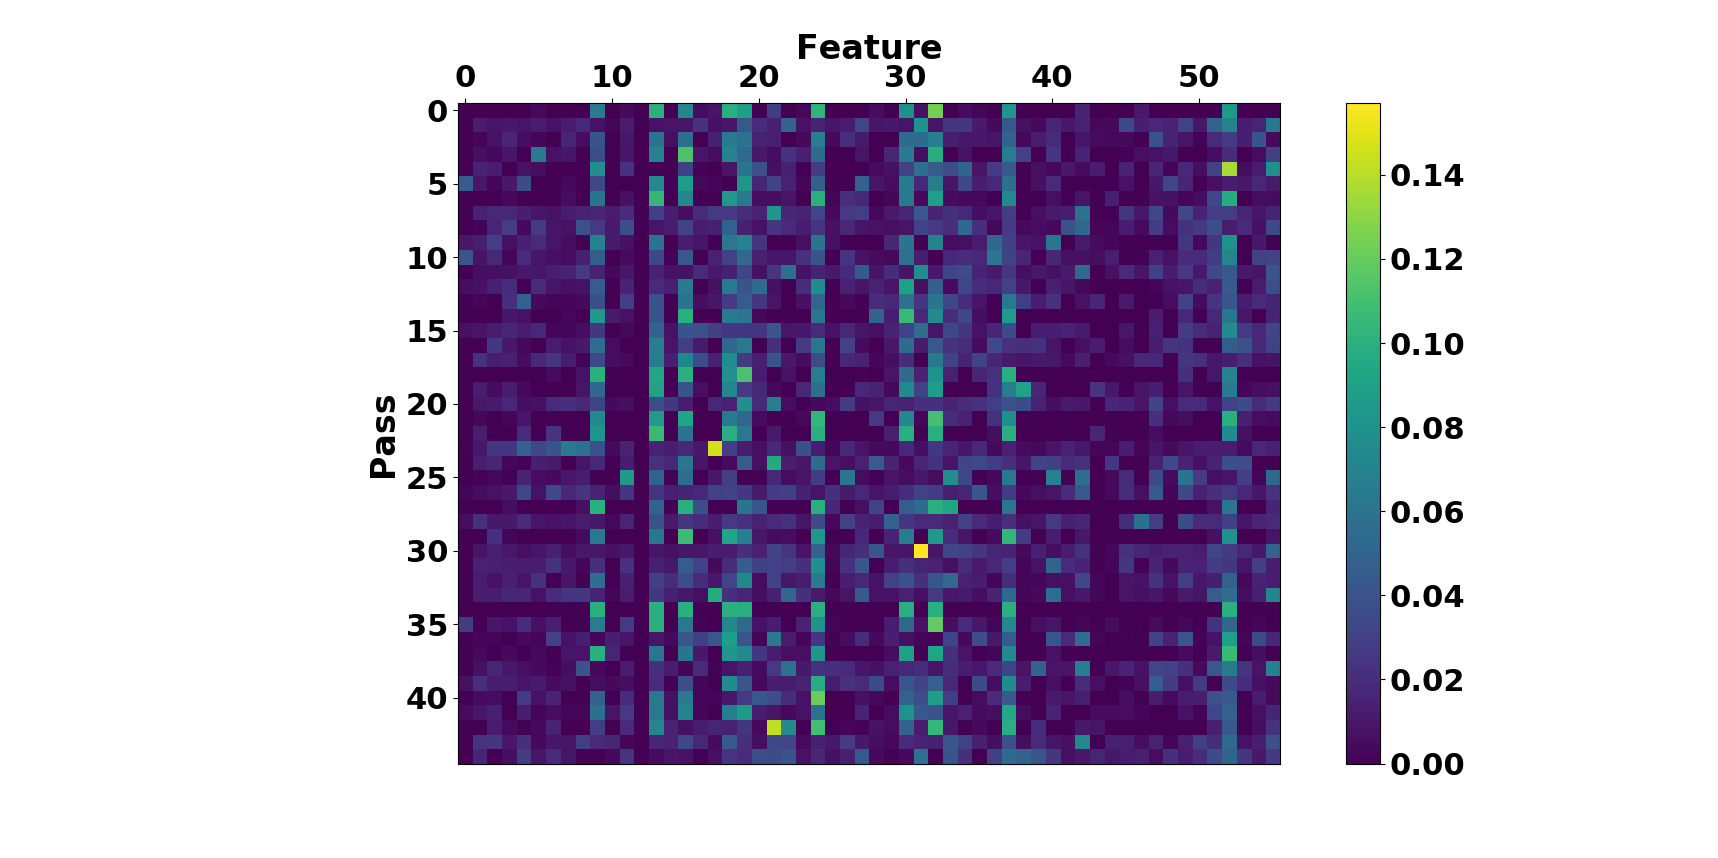
\includegraphics[trim={9cm 3.5cm 4.2cm 0.8cm},clip,width=0.5\textwidth]{Figures/randforest.png}
    \caption{Heat map illustrating the importance of feature and pass indices.}
    \label{fig:heatmap1}
    \vspace{-0.1cm}
\end{figure}

Other expected behaviors are also observed in this figure. For instance, the correlation between \textit{number of branches} and the transform passes \textit{-loop-simplify}, \textit{-tailcallelism} (which transforms calls of the current function \textit{i.e.}, self recursion, followed by a return instruction with a branch to the entry of the function, creating a loop), \textit{-lowerswitch} (which rewrites switch instructions with a sequence of branches). Other interesting behaviors are also captured. For example, in the correlation between \textit{binary operations with a constant operand} and \textit{-functionattrs}, which marks different operands of a function as read-only (constant). 
Some correlations are harder to explain, for example, \textit{number of BitCast instructions} and \textit{-instcombine}, which combines  instructions into fewer simpler instructions. This is actually a result of \textit{-instcombine} reducing the loads and stores that call bitcast instructions for casting pointer types.  
%Apparently, in some cases, \textit{-instcombine} checks for the types and turns instructions with undefined behavior into unreachable, which directly lowers the number of BitCast instructions. 
Another example is \textit{number of memory instructions} and \textit{-sink}, where \textit{-sink} basically moves memory instructions into successor blocks and delays the execution of memory until needed.  Intuitively, whether to apply \textit{-sink} should be dependent on whether there is any memory instruction in the program. 
Our last example to show is \textit{number of occurrences of constant 0} and \textit{-deadargelim}, where \textit{-deadargelim} helped eliminate dead/unused constant zero arguments. 


Overall, we observe that all the passes % except for pass number 26 (\textit{-early-cse}) 
are correlated to some features and are able to affect the final circuit performance. 
%a transformation of the program in a way that could improve or worsen its performance. %Pass \textit{-early-cse} was not very helpful because only a small fraction of the programs tested had trivially redundant computations that could be eliminated. Note that this was not the case for CHstone; in CHstone all the passes were useful, because CHstone includes a wide range of applications in different domains.
We also observe that multiple features are not effective at directing decisions and training with them could increase the variance that would result in lower prediction accuracy of our results. 
For example, the total number of instructions did not give a direct indication of whether applying a pass would be helpful or not. This is because sometimes more instructions could improve the performance (for example, due to loop unrolling) and eliminating unnecessary code could also improve the performance. In addition, the importance of features varies among different benchmarks depending on the tasks they perform.
\vspace{-0.2cm}
\subsection{Importance of Previously Applied Passes}
\begin{figure}[!t]
    \centering
    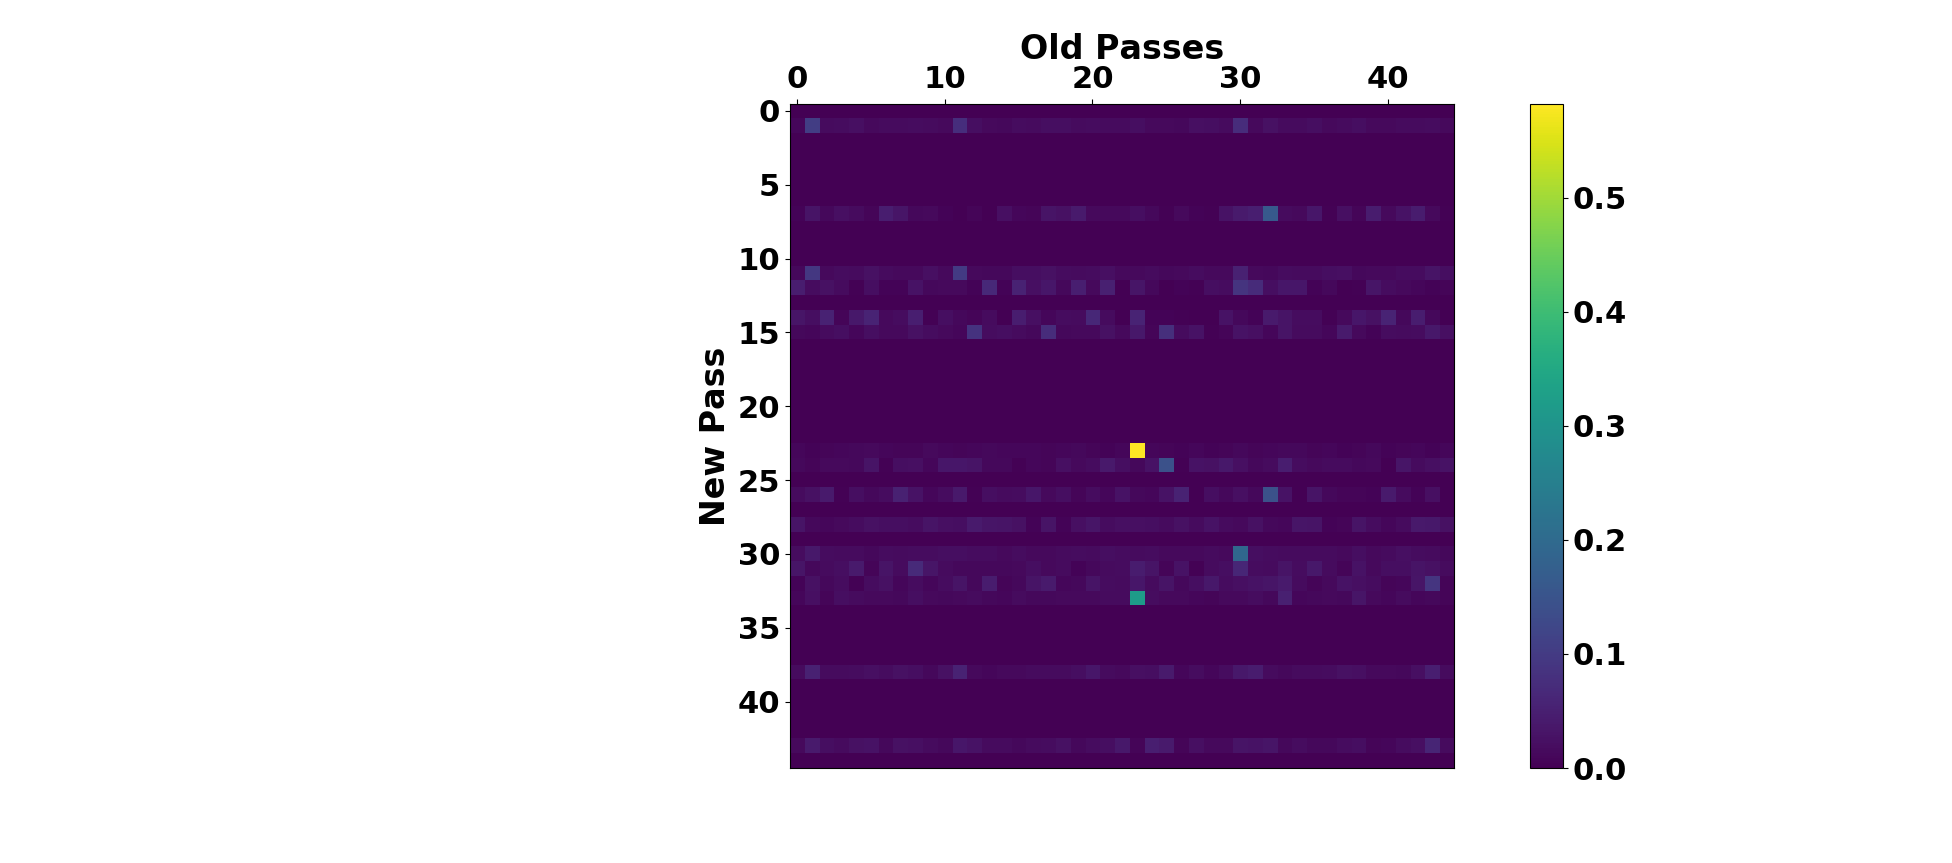
\includegraphics[trim={15cm 3.5cm 4.6cm 0.8cm},clip,width=0.5\textwidth]{Figures/tree3.png}
    \caption{Heat map illustrating the importance of indices of previously applied passes and the new pass to apply.}
    \label{fig:heatmap2}
\end{figure}

Figure~\ref{fig:heatmap2} illustrates the impact of previously applied passes on the new pass to apply. The higher the value is, the more important having the old pass is. From this figure, we learn that for the programs we trained on passes \textit{-scalarrepl, -gvn, -scalarrepl-ssa, -loop-reduce, -loop-deletion, -reassociate, -loop-rotate, -partial-inliner, -early-cse, -adce, -instcombine, -simplifycfg, -dse, -loop-unroll, -mem2reg, and -sroa}, are more impactful on the performance compared to the rest of the passes regardless of their order in the trajectory. Point (23,23) has the highest importance in which implies that pass \textit{-loop-rotate} is very helpful and should be included if not applied before. By examining thousands of the programs, we find that \textit{-loop-rotate} indeed reduces the cycle count significantly. Interestingly, applying this pass twice is not harmful if the passes were given consecutively. However, giving this pass twice with some other passes between them is sometimes very harmful. Another interesting behavior our heat map captured is the fact that applying pass 33 (\textit{-loop-unroll}) after (not necessarily consecutive) pass 23 (\textit{-loop-rotate}) was much more useful compared to applying these two passes in the opposite order. 